\documentclass[11pt]{article}
%Gummi|065|=)
\usepackage[top=1in, bottom=1in, left=0.5in, right=0.5in]{geometry}
\usepackage{graphicx}
\title{Project Report}
\author{Venkata Dinesh (120050051)\\
\texttt {dineshkota3@cse.iitb.ac.in}\and
Nitish Chandra (120050071)\\
\texttt{nitish@cse.iitb.ac.in}\and
Kota Mahindar (120050073)\\
\texttt{mahindar@cse.iitb.ac.in}
}
\date{}
\begin{document}
\maketitle
\section*{Original design vs Finished design}
\subsection*{Original design}
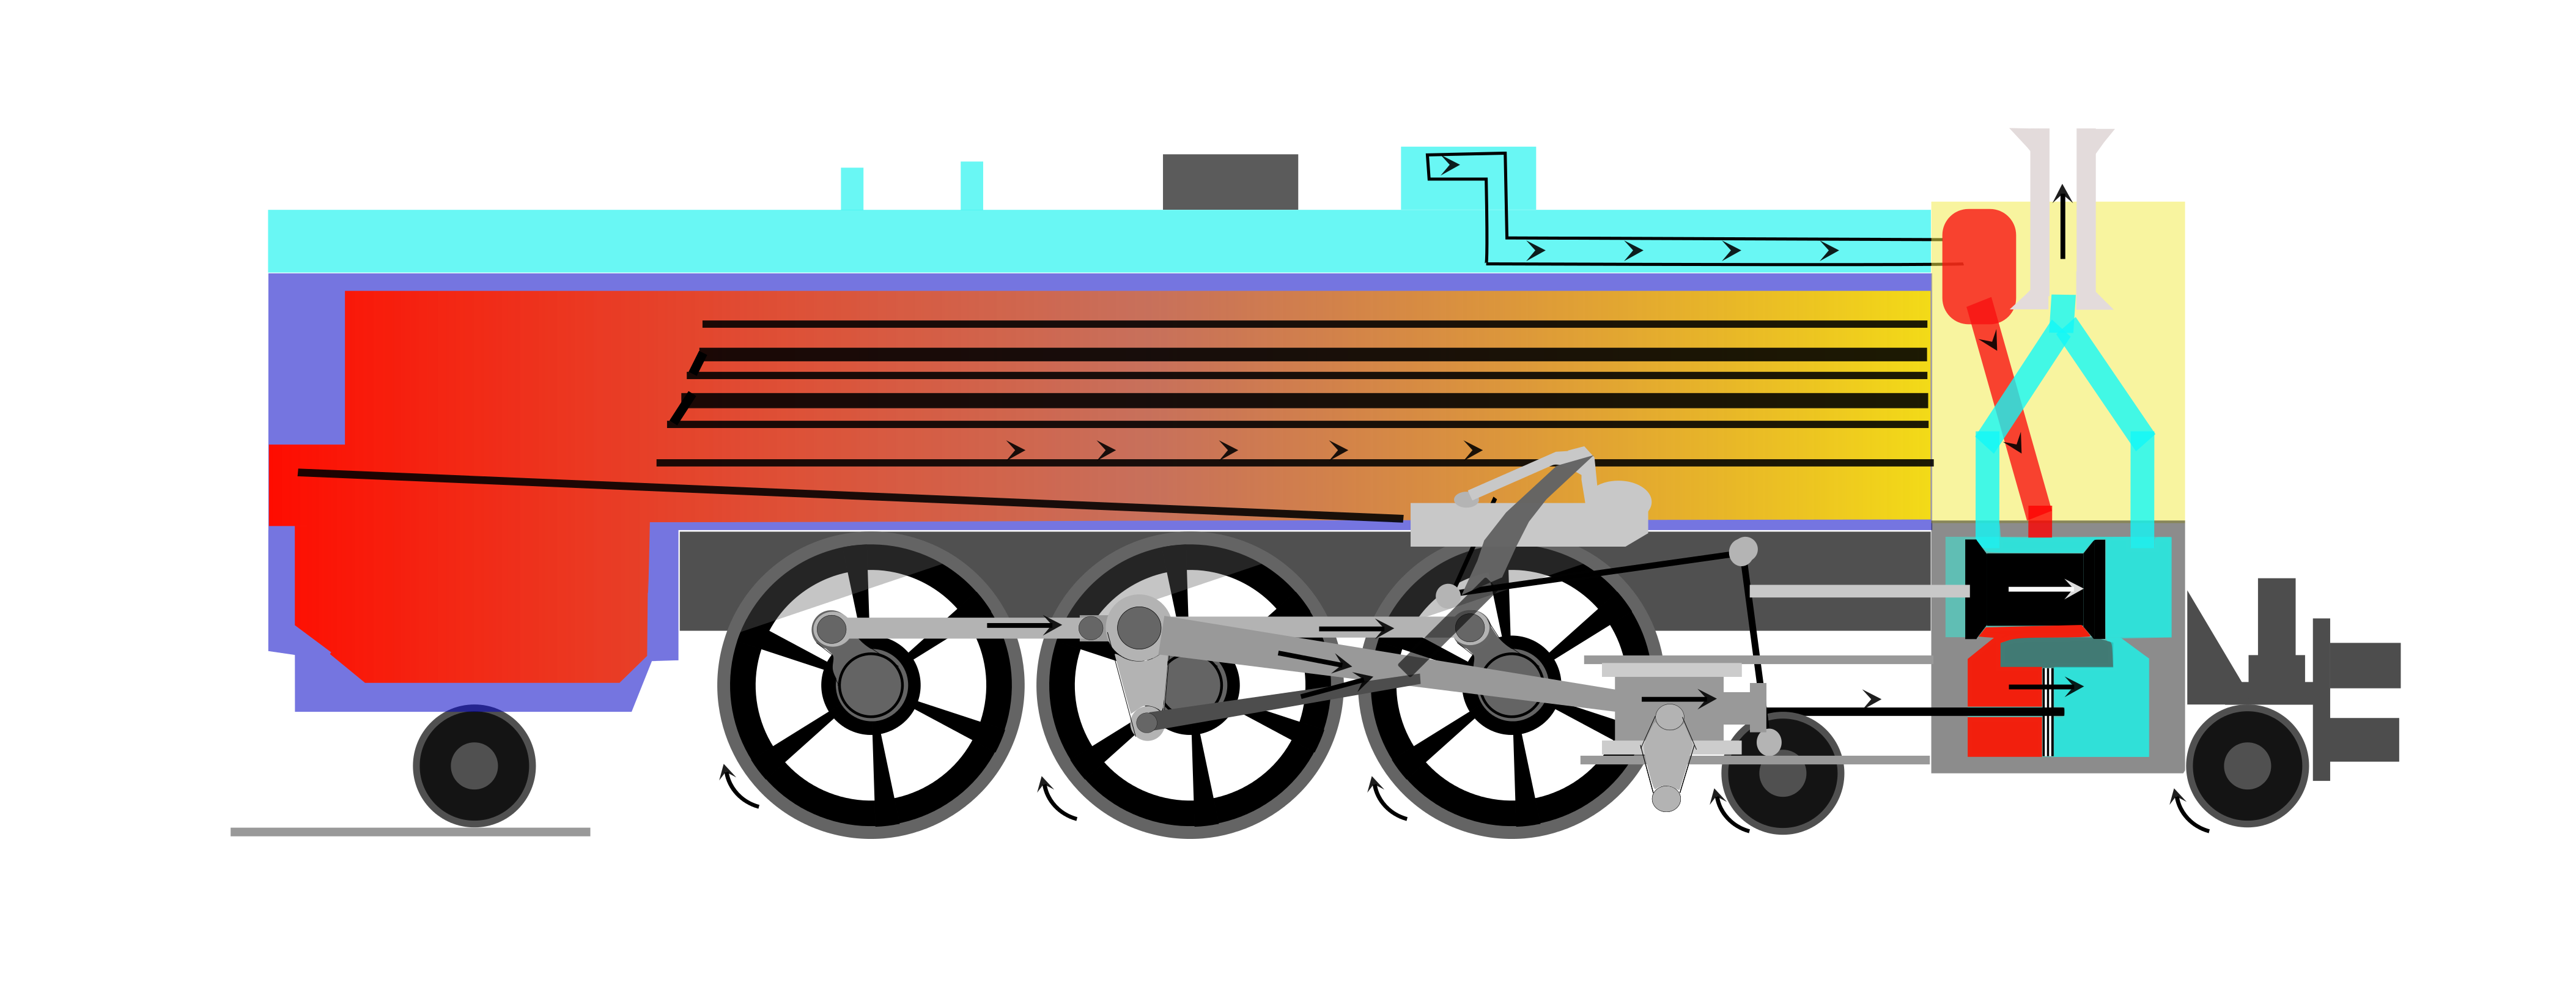
\includegraphics[scale = 0.1]{project.png}
\subsection*{Final design}
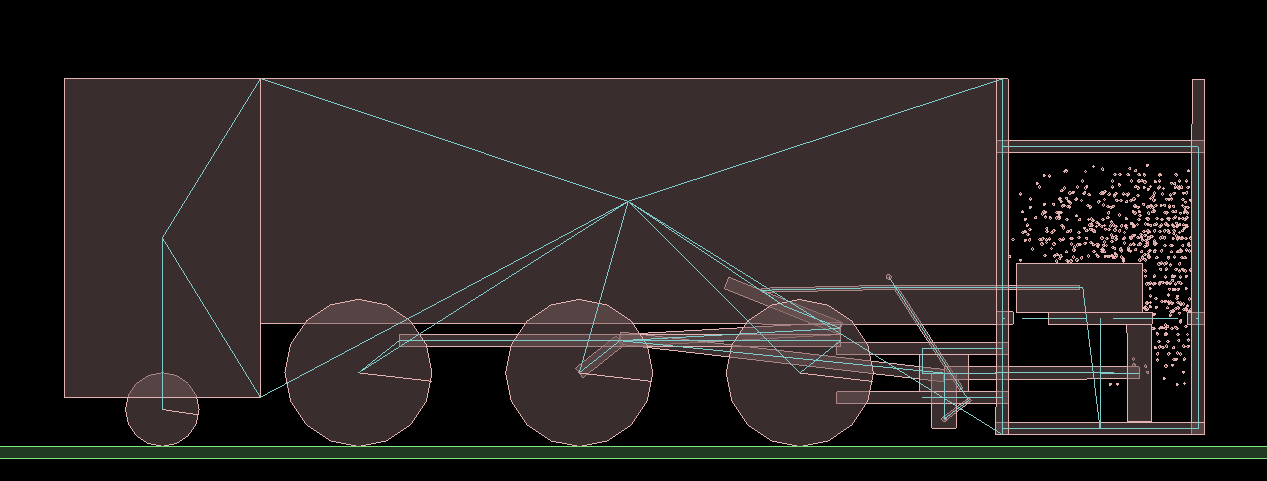
\includegraphics[scale = 0.3]{newtrain.png}
\subsection*{Deviations}
\begin{enumerate}
\item Unnecessary blocks at the top of train, spokes of wheels have been removed because they don't add to the physics of Steam Engine
\item Outlet for steam are not included 
\item Steam has been approximated with small circles constructed using {\tt b2CircleShape}. This is because, Box2D allows only rigid bodies. So, to represent fluids like steam, we need to approximate them with small rigid bodies.
\item We cannot represent temperature changes in Box2D. So, it is difficult to move gas particles produced at the end of engine to the start of engine without temperature gradient. So, steam is created at the front of engine.
\end{enumerate}

\section*{Interesting things}
We included three keyboard shortcuts to control the motion of steam engine.
\begin{itemize}
\item {\tt b} : Apply breaks 
\item {\tt q} :
Accelerate train by applying force on piston 
\item {\tt c} :
To create more steam and thus accelerate the steam engine.
\end{itemize}
\subsubsection*{Special arrangement of blocks}
\centerline{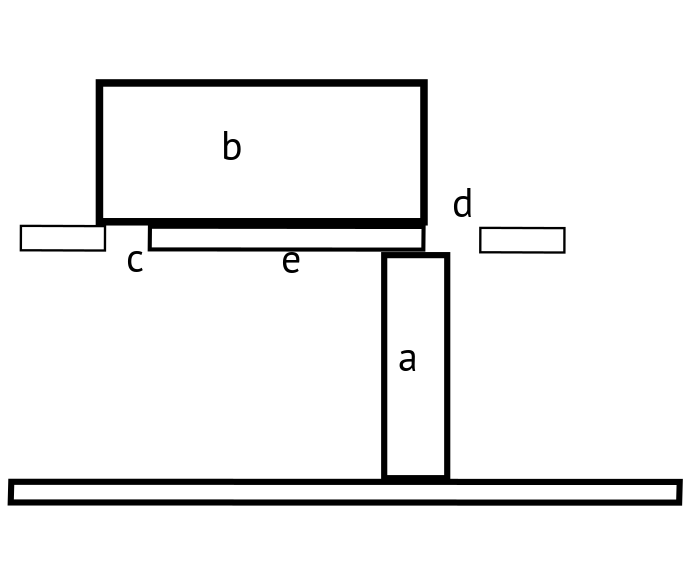
\includegraphics[scale = 0.3]{drawing.png} }
Let the above diagram show the arrangement of piston at the front of steam engine. Pistons {\it a} and {\it b} move whenever steam particles collide with them. Due to the arrangement of bodies to the left of these pistons, these two bodies always travel in opposite directions. This ensures that whenever piston {\it a} reaches the right end of block {\it e}, hole {\it c} is closed and steam starts entering from {\it d} making {\it a} to travel backwards.

Similarly, whenever {\it a} reaches hole {\it c}, it is pushed towards right.  

\subsubsection*{Approximating temperature effect}
\centerline{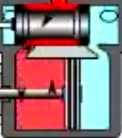
\includegraphics{temperature.png}}
In the diagram shown above, particles to the left of piston {\it a} (shown in red), are of higher temperature and thus impart a larger velocity to piston whereas particles to right of {\it a}, are of lower temperature and thus impart very low velocity to piston.

To simulate this effect, we made the following arrangement.

Suppose piston {\it a} is moving to right. This means that gas particles on left side have higher temperature. So, potentially, only the particles to left of it can impart considerable velocity to it. 

\centerline{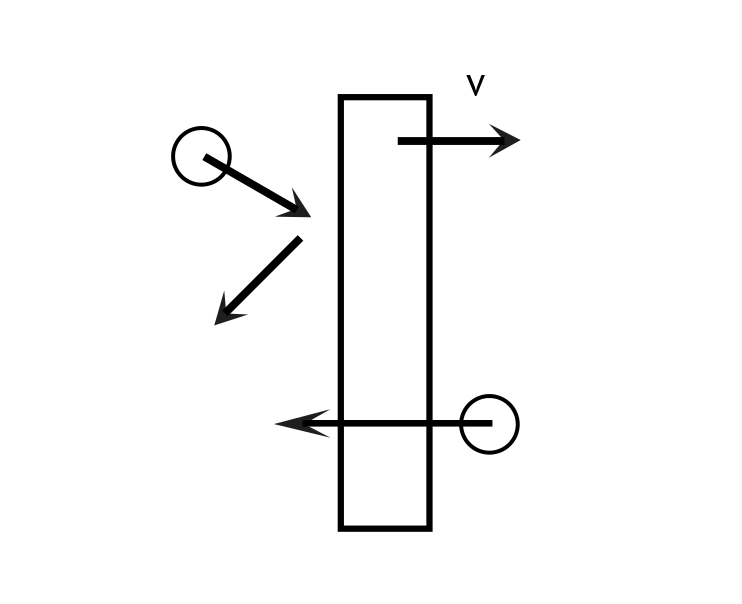
\includegraphics[scale = 0.2]{collision.png}} 

We can simulate the same situation assuming that particles to the right of it don't collide at all. Such an arrangement can be made using {\tt PreSolve} function in {\tt cs296\_base.cpp}\cite{OneSidedPlatform.h}
\subsubsection*{Simulating Outlet}
In reality, particles which have lost their temperature due to repeated collisions and dissipation of energy go out through outlet. Even without the temperature, we can use the velocities of particles to detect when to oust them. We fixed a minimum value of velocity of particles(w.r.t train) so that if any particle has a speed less than minimum, the program destroys the particle. This is similar to throwing out the particles of lower temperature.

\subsubsection*{Stacking of objects}
We can see that, many objects overlap with wheels of train. This usually leads to collision between overlapping objects (because their AABBs overlap). But, in case of real steam engine, rods lie {\it in front of} wheels. Since Box2D cannot deal with objects in 3D, we cannot ensure that there is a difference in {\it z} component of the objects. So, in 2D, we have to overlap objects and still ensure that they don't collide with each other. We did this using {\tt groupIndex} and {\tt maskBits, categoryBits}\cite{man}.

\section*{Results of Profiling}
We compared the results after profiling our simulation in release profile and debug profile
We compared the profiles for iteration number 200000. Highest amount of time is consumed by the function {\tt operation-(b2Vec2 const\&, b2Vec2 const\&)}.This is due to the fact that it involves a lot of vector calculations.

These results for {\tt Release} profiling were obtained using {\tt -O3} flag.


Following are the profiling results for some functions that have been modified



{\tt 
0.00   0.00        2     0.00    10.01  cs296::base\_sim\_t::base\_sim\_t()

0.00   0.00        2     0.00    10.01  cs296::base\_sim\_t::base\_sim\_t()

\vskip 0.2in

0.00   0.00        1     0.00    10.07  cs296::dominos\_t::dominos\_t()

0.00   0.00        1     0.00    30.01  cs296::dominos\_t::dominos\_t()
}
{}

Where first row indicates results with {\tt Release} flag and second row indicates results with {\tt Debug} flag and columns indicate \% of total time spent, self time spend in total function calls, self time spent per call in {\tt ms}, total time spent per call in {\tt ms}

We can see that {\tt base\_sim\_t()} is optimised. But {\tt dominos\_t()} where the entire creation of bodies takes place takes more amount of time with {\tt Debug} flag.

With respect to remaining methods, both the profiles have approximately same running times.

This is also evident from Call Graphs


\includegraphics[width=7.7in, height=2in]{debug.png}


\includegraphics[width=7.7in, height=2in]{release.png}

\subsection*{Analysis of the Plots}
These plots have been generated using 100 iterations and 30 reruns.

\centerline{
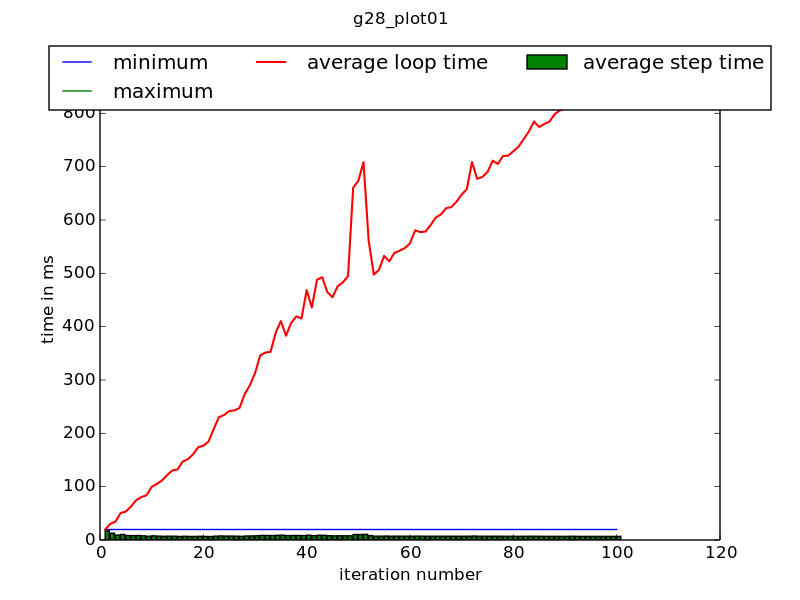
\includegraphics[scale = 0.5]{g28_plot01.png}
}

From Plot1 we can observe that {\bf loop time} increases with increasing iteration value. Since with increase in iteration value, we also increase the number of times the loop runs, it is natural for the {\bf loop time} to increase with the iteration value. 

\centerline{
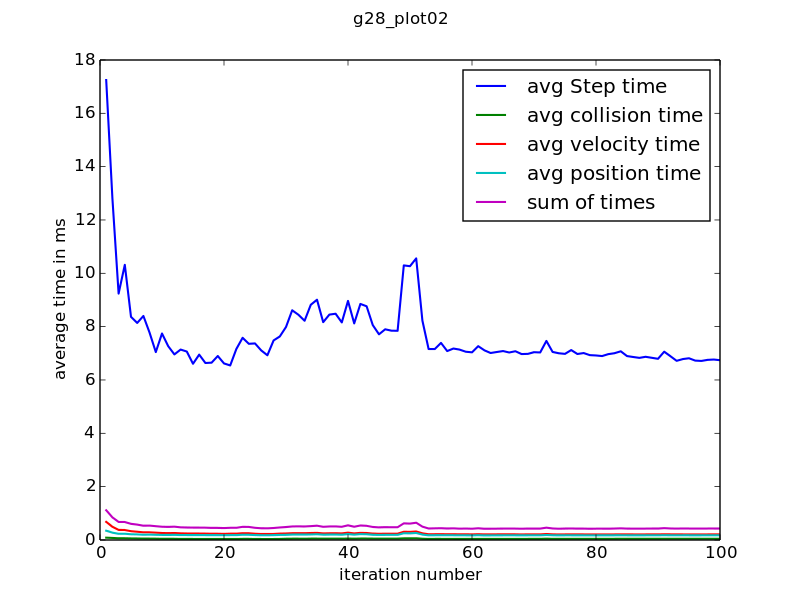
\includegraphics[scale = 0.5]{g28_plot02.png}
}


From Plot2 we observe that {\bf collision time, velocity time, position time} decrease with increase in iteration value. This is because collision time is the time taken by program to detect the collision, find the values of collision parameters etc.. To find these values, some subroutines are invoked. When these functions are called, kernel sometimes interrupts the process to allocate time for other processes. So, this interruption time is included in {\bf collision time}.  By observing the data, we can conclude that the increase in total interruption time with iteration number is very less.
$$average collision time = \left(\sum c_i +  total interruption time\right)/v$$ where $v$ is the number of iterations and $c_i$ is the collision time for $i$th iteration. Since the rate of increase of total interruption time  is $<<$ 1, and $c_i$ is nearly same except for the instances when collision happens and these instances occur with a gap of many iteration values, average collision time decreases with increase in iteration value.
 
Similar reason explains the decreasing trend of {\bf velocity time, position time} with respect to iteration value.


We can observe from Plot1 that the average {\bf steptime} is decreasing with increasing iteration number. From Plot2 we can observe that sum of {\bf collision time, position time, velocity time} is strictly less than {\bf step time}, the reason being {\bf step time} includes the time taken to calculate positions, velocities, collision parameters for the next step and also time for which this program is interrupted by kernel. Since all the parameters decrease with increase in iteration value, {\bf step time} also decreases with iteration number.


\centerline{
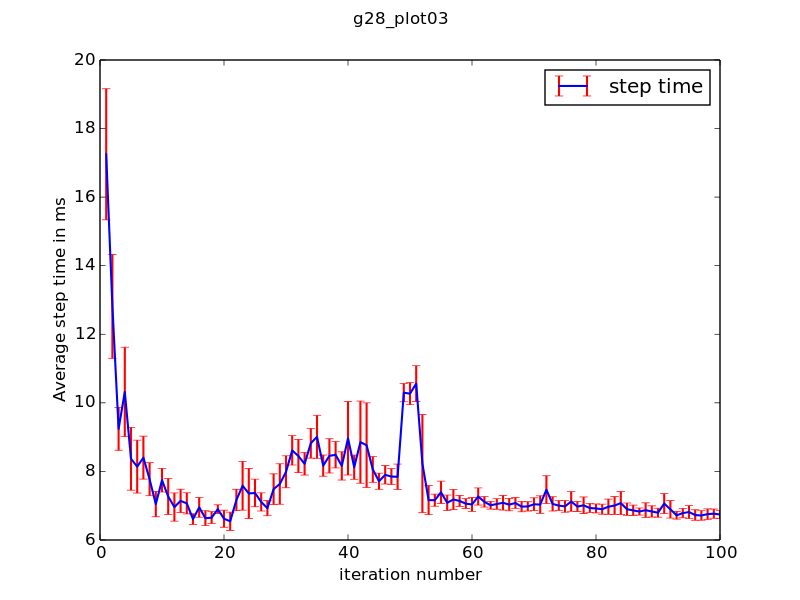
\includegraphics[scale = 0.5]{g28_plot03.png}
}


From the above plot, we can observe that,as the {\bf step time} decreases, error in step time also decreases. The error in {\bf step time} arises because, total interruption time usually varies with time. As the iteration value increases, both the average {\bf step time} and average interruption time decrease, so the error associated with {\bf step time}
also decreases.


\section*{Drawbacks}
If the number of steam particles are too high then there is a distortion among objects in the front part of train and the joint's conditions may not be preserved. Due to their greater number the functions related to the collisions may take more amount of time, so there will be considerable slowdown of simulation.




\bibliographystyle{plain}
\bibliography{report}
\end{document}